\documentclass[12pt]{article}
\usepackage{amsmath}
\usepackage{graphicx}
\usepackage{geometry}
\usepackage{tikz} % Added for drawing diagrams
\geometry{a4paper, margin=1in}

\title{Magnetic Fields: 1-Hour Lesson Notes}
\author{}
\date{}

\begin{document}

\maketitle

These notes cover the core concepts of magnetic fields, focusing on the forces they exert and the fields they create.

\section{Magnetic Force on a Moving Charge}

A magnetic field, denoted by $\vec{B}$, exerts a force on a moving electric charge. This is the fundamental interaction.

\begin{itemize}
    \item \textbf{Key Idea:} Magnetic fields only affect \textbf{moving} charges.
    \item \textbf{The Lorentz Force Law:} The magnetic force $\vec{F}_B$ on a charge $q$ moving with velocity $\vec{v}$ in a magnetic field $\vec{B}$ is given by:
    \begin{equation*}
        \vec{F}_B = q(\vec{v} \times \vec{B})
    \end{equation*}
    \item \textbf{Magnitude of the Force:} The size of the force is $F_B = |q|vB\sin\theta$, where $\theta$ is the angle between the velocity $\vec{v}$ and the magnetic field $\vec{B}$. The force is \textbf{maximum} when they are perpendicular ($\theta = 90^\circ$) and \textbf{zero} when they are parallel ($\theta = 0^\circ$).
    \item \textbf{Direction (Right-Hand Rule):}
    \begin{enumerate}
        \item Point your fingers in the direction of velocity $\vec{v}$.
        \item Curl your fingers towards the direction of the magnetic field $\vec{B}$.
        \item Your thumb points in the direction of the force $\vec{F}_B$ for a \textbf{positive charge}.
        \item If the charge is \textbf{negative}, the force is in the \textbf{opposite} direction of your thumb.
    \end{enumerate}
    \item \textbf{Circular Motion:} Because the magnetic force is always perpendicular to the velocity, it acts as a centripetal force, causing the charged particle to move in a circle (if $\vec{v}$ is perpendicular to a uniform $\vec{B}$).
    \begin{itemize}
        \item \textbf{Centripetal Force:} $F_c = \frac{mv^2}{r}$
        \item \textbf{Equating Forces:} $qvB = \frac{mv^2}{r}$
        \item \textbf{Radius of Path:} $r = \frac{mv}{qB}$
    \end{itemize}
\end{itemize}

\subsection*{Calculation Example}
A proton ($m = 1.67 \times 10^{-27}$ kg, $q = +1.6 \times 10^{-19}$ C) moves at $2.0 \times 10^6$ m/s perpendicularly into a uniform magnetic field of $0.5$ T.
\begin{itemize}
    \item \textbf{Force:} $F = qvB\sin(90^\circ) = (1.6 \times 10^{-19})(2.0 \times 10^6)(0.5)(1) = 1.6 \times 10^{-13}$ N.
    \item \textbf{Radius:} $r = \frac{mv}{qB} = \frac{(1.67 \times 10^{-27})(2.0 \times 10^6)}{(1.6 \times 10^{-19})(0.5)} = 0.042$ m or 4.2 cm.
\end{itemize}

\section{Magnetic Force on a Current-Carrying Wire}

A current is just a collection of moving charges, so a wire with current $I$ also experiences a force in a magnetic field.

\begin{itemize}
    \item \textbf{Formula:} For a straight wire of length $L$, the force is:
    \begin{equation*}
        \vec{F}_B = I(\vec{L} \times \vec{B})
    \end{equation*}
    where $\vec{L}$ is a vector pointing in the direction of the current.
    \item \textbf{Magnitude:} $F_B = ILB\sin\theta$.
\end{itemize}

\subsection*{Calculation Example}
A 0.50 m wire carrying 5.0 A of current is placed in a 0.50 T magnetic field at an angle of $90^\circ$.
\begin{itemize}
    \item \textbf{Force:} $F = ILB\sin(90^\circ) = (5.0)(0.50)(0.50)(1) = 1.25$ N.
\end{itemize}

\section{Sources of Magnetic Fields}

Moving charges and currents don't just \textit{feel} magnetic fields; they also \textit{create} them.

\begin{itemize}
    \item \textbf{Current Loop:} A circular loop of wire with radius $R$ carrying current $I$ creates a magnetic field at its center with magnitude:
    $$B = \frac{\mu_0 I}{2R}$$
    where $\mu_0 = 4\pi \times 10^{-7}$ T·m/A is the permeability of free space.
    \item \textbf{Long Straight Wire:} The field at a distance $r$ from a long, straight wire carrying current $I$ is:
    $$B = \frac{\mu_0 I}{2\pi r}$$
\end{itemize}

\section{Torque on a Current Loop (Magnetic Dipoles)}

When a current loop is placed in a uniform magnetic field, it experiences a torque that tries to align it with the field.

\begin{itemize}
    \item \textbf{Magnetic Dipole Moment ($\vec{\mu}$):} A property of a current loop. For a flat loop with $N$ turns, area $A$, and current $I$:
    \begin{itemize}
        \item \textbf{Magnitude:} $\mu = NIA$
        \item \textbf{Direction:} Perpendicular to the plane of the loop (given by a right-hand rule: curl fingers with the current, thumb points in the direction of $\vec{\mu}$).
    \end{itemize}
    \item \textbf{Torque ($\vec{\tau}$):} The torque on the loop is:
    \begin{equation*}
        \vec{\tau} = \vec{\mu} \times \vec{B}
    \end{equation*}
    \begin{itemize}
        \item \textbf{Magnitude:} $\tau = \mu B \sin\theta$, where $\theta$ is the angle between $\vec{\mu}$ and $\vec{B}$.
    \end{itemize}
    \item \textbf{Potential Energy ($U$):} The potential energy of the dipole in the field is:
    \begin{equation*}
        U = -\vec{\mu} \cdot \vec{B} = -\mu B \cos\theta
    \end{equation*}
    The loop is most stable at its lowest energy state ($\theta = 0^\circ$, when $\vec{\mu}$ aligns with $\vec{B}$).
\end{itemize}

\newpage
\section{Solved Problems from PDFs}

\subsection{Problem 1 (Bohr Model \& Spinning Disc)}
\textbf{Question Source:} SPhO 2019 Theory Paper 2 (Bfield5.pdf)

\subsubsection*{(i) Bohr's Hydrogen Atom}
\textbf{Question:} (i) According to Bohr's theory, when the hydrogen atom is in its ground state, the electron is revolving around the proton in circular orbit with a radius of $5.3\times10^{-10}$ m. The speed of the electron in its orbit is $6.91\times10^{5}ms^{-1}$ Determine the magnitude of the magnetic field at the position of the proton due to the orbital motion of the electron.

\textbf{Explanation:} The orbiting electron acts like a tiny current loop. We can find the equivalent current $I$ and then use the formula for the magnetic field at the center of a current loop. 
\textit{Note: The solution below uses the standard Bohr radius of $5.3 \times 10^{-11}$ m, as the value of $5.3 \times 10^{-10}$ m in the problem text is likely a typo and inconsistent with the ground state.}

\textbf{Solution:}
\begin{enumerate}
    \item \textbf{Find the period of revolution ($T$):} The time for one full circle.
    $$T = \frac{\text{circumference}}{\text{speed}} = \frac{2\pi r}{v}$$
    \item \textbf{Find the equivalent current ($I$):} Current is charge per unit time. In one period, a charge of $e$ passes any point in the orbit.
    $$I = \frac{q}{T} = \frac{e}{2\pi r / v} = \frac{ev}{2\pi r}$$
    \item \textbf{Calculate the magnetic field ($B$):} Use the formula for the center of a current loop.
    $$B = \frac{\mu_0 I}{2r} = \frac{\mu_0}{2r} \left(\frac{ev}{2\pi r}\right) = \frac{\mu_0 e v}{4\pi r^2}$$
    \item \textbf{Substitute the values:} (Using $r = 5.3 \times 10^{-11}$ m)
    \begin{align*}
        B &= \frac{(4\pi \times 10^{-7} \, \text{T·m/A})(1.60 \times 10^{-19} \, \text{C})(6.91 \times 10^5 \, \text{m/s})}{4\pi (5.3 \times 10^{-11} \, \text{m})^2} \\
        B &\approx 3.93 \, \text{T}
    \end{align*}
\end{enumerate}

\subsubsection*{(ii) Spinning Disc}
\textbf{Question:} (ii) A circular disc has a radius R and surface charge density $\sigma$. It is spinning at n revolutions per second. What is the magnetic field at the centre of the disc?

\textbf{Explanation:} We can think of the disc as a collection of infinitesimally thin concentric rings. We'll find the magnetic field from one ring and then integrate over the entire disc.

\textbf{Solution:}
\begin{enumerate}
    \item \textbf{Consider a thin ring:} Take a ring at radius $r$ with thickness $dr$.
    \item \textbf{Charge of the ring ($dq$):} The area of the ring is $dA = 2\pi r dr$. The charge is $dq = \sigma \cdot dA = \sigma (2\pi r dr)$.
    \item \textbf{Current of the ring ($dI$):} The ring spins $n$ times per second (frequency). The period is $T=1/n$. So, the equivalent current is $dI = \frac{dq}{T} = dq \cdot n = 2\pi\sigma n r dr$.
    \item \textbf{Magnetic field from the ring ($dB$):} The field at the center due to this ring is:
    $$dB = \frac{\mu_0 dI}{2r} = \frac{\mu_0 (2\pi\sigma n r dr)}{2r} = \mu_0 \pi \sigma n dr$$
    \item \textbf{Integrate to find total B:} Sum the fields from all rings from the center ($r=0$) to the edge ($r=R$).
    \begin{align*}
        B &= \int_0^R dB = \int_0^R \mu_0 \pi \sigma n dr = \mu_0 \pi \sigma n \int_0^R dr \\
        B &= \mu_0 \pi \sigma n [r]_0^R = \mu_0 \pi \sigma n R
    \end{align*}
\end{enumerate}

\newpage
\subsection{Problem 2 (Proton Beam Deflection)}
\textbf{Question Source:} SPhO 2020 Theory Paper (Bfield2.pdf)

\textbf{Question:} A beam of proton with kinetic energy 10 MeV is travelling in the positive x-direction. It enters a magnetic field of magnitude 1.5 T and the direction of the magnetic field is in the positive z-direction. The magnetic field extends from $x=0$ to $x=2.0$ m as shown in Fig. 1. Determine the angle $\alpha$ between the initial velocity vector of the proton beam and the velocity vector after the beam emerges from the magnetic field.

\begin{figure}[h]
\centering
% CORRECTED TikZ drawing for Figure 1
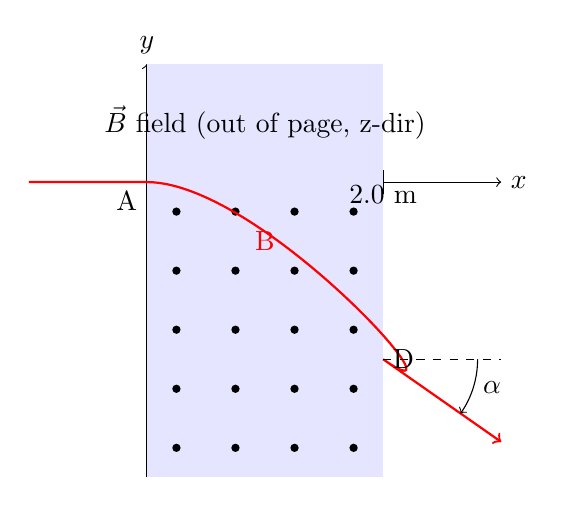
\begin{tikzpicture}[scale=1.5]
    % Draw axes
    \draw[->] (-1, 0) -- (3, 0) node[right] {$x$};
    \draw[->] (0, -2.5) -- (0, 1) node[above] {$y$};
    
    % Shaded B-field region
    \fill[blue!10] (0, -2.5) rectangle (2, 1);
    \node at (1, 0.5) {$\vec{B}$ field (out of page, z-dir)};
    \foreach \x in {0.25, 0.75, 1.25, 1.75}
        \foreach \y in {-2.25, -1.75, -1.25, -0.75, -0.25}
            \fill (\x, \y) circle (1pt);
    \draw (2, -0.1) -- (2, 0.1) node[below=2pt] {$2.0$ m};
    \node at (0,0) [below left] {A};
    
    % Particle Path (as shown in PDF, curving down)
    % This is now one continuous path
    \draw[->, thick, red] (-1, 0) -- (0, 0) to[out=0, in=325] (2, -1.5) -- (3, -2.2);
    \node at (2, -1.5) [right] {D};
    \node at (1, -0.5) [red] {B};
    
    % Angle alpha
    \draw[dashed] (2, -1.5) -- (3, -1.5);
    \draw[->] (2.8, -1.5) arc (0:-35:0.8) node[midway, right] {$\alpha$};
\end{tikzpicture}
\caption{Figure 1 from SPhO 2020 Theory Paper.}
\end{figure}

\textbf{Explanation:} The proton will travel along the arc of a circle while inside the magnetic field. The angle of deflection $\alpha$ can be found using trigonometry once we determine the radius of this circular path.
Note: The given values lead to a non-physical result where the proton completes a full semi-circle within the field. The solution proceeds by calculating this outcome.

\textbf{Solution:}
\begin{enumerate}
    \item \textbf{Convert Kinetic Energy (KE) to Joules:}
    $$\text{KE} = 10 \, \text{MeV} = 10 \times 10^6 \times (1.6 \times 10^{-19} \, \text{J/eV}) = 1.6 \times 10^{-12} \, \text{J}$$
    \item \textbf{Find the proton's momentum ($p$):} We know $\text{KE} = \frac{p^2}{2m}$, so $p = \sqrt{2m(\text{KE})}$.
    $$p = \sqrt{2(1.67 \times 10^{-27} \, \text{kg})(1.6 \times 10^{-12} \, \text{J})} = 7.31 \times 10^{-20} \, \text{kg·m/s}$$
    \item \textbf{Calculate the radius of the circular path ($R$):}
    $$R = \frac{mv}{qB} = \frac{p}{qB} = \frac{7.31 \times 10^{-20} \, \text{kg·m/s}}{(1.6 \times 10^{-19} \, \text{C})(1.5 \, \text{T})} = 0.3046 \, \text{m}$$
    \item \textbf{Determine the angle $\alpha$:}
    The diameter of the proton's path is $2R = 2(0.3046 \, \text{m}) = 0.6092 \, \text{m}$.
    Since the magnetic field extends for $2.0$ m, which is much wider than the diameter of the path, the proton will complete a full semi-circle and exit the field moving in the opposite direction.
    Therefore, the angle between the initial and final velocity vectors is $180^\circ$ or $\pi$ radians.
\end{enumerate}

\subsection{Problem 3 (Velocity Filter)}
\textbf{Question Source:} SPhO 2019 Theory Paper 1 (Bfield4.pdf)

\textbf{Question:} (i) If the spectrometer were used with $100~\text{Vcm}^{-1}$ between the plates and a magnetic field of 0.2 T, what would be the speed of an ion that can pass through the velocity filter?

\textbf{Explanation:} A velocity filter uses perpendicular electric ($\vec{E}$) and magnetic ($\vec{B}$) fields. It's designed so that only particles of a specific velocity pass through undeflected. This happens when the magnetic force ($F_B = qvB$) exactly balances the electric force ($F_E = qE$).

\textbf{Solution:}
\begin{enumerate}
    \item \textbf{Set the forces equal:} For the ion to pass straight through, $F_B = F_E$.
    $$qvB = qE$$
    \item \textbf{Solve for velocity ($v$):}
    $$v = \frac{E}{B}$$
    \item \textbf{Convert units:} The electric field is given as $E = 100 \, \text{V/cm}$.
    $$E = 100 \frac{\text{V}}{\text{cm}} \times \frac{100 \text{ cm}}{1 \text{ m}} = 10000 \, \text{V/m}$$
    \item \textbf{Calculate the speed:}
    $$v = \frac{10000 \, \text{V/m}}{0.2 \, \text{T}} = 50000 \, \text{m/s} = 5.0 \times 10^4 \, \text{m/s}$$
\end{enumerate}

\newpage
\subsection{Problem 4 (Torque on a Loop)}
\textbf{Question Source:} SPhO 2024 Theory Paper (Bfield1.pdf)

\begin{figure}[h]
\centering
% CORRECTED TikZ drawing for Figure 6
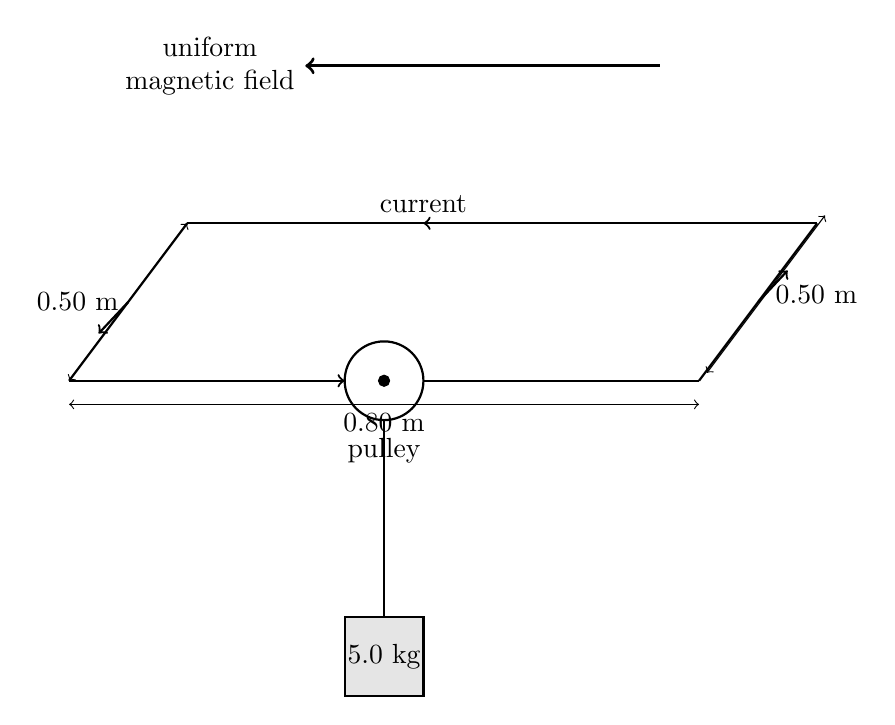
\begin{tikzpicture}[scale=1]
    % The B-field
    \draw[->, very thick] (4.5, 2.5) -- (0, 2.5) node[left, align=center] {uniform \\ magnetic field};
    
    % The loop (in perspective)
    % Front arm (0.80 m) - This is the axis
    \draw[thick, fill=gray!30] (-3, -1.5) -- (5, -1.5);
    % Back arm (0.80 m)
    \draw[thick] (-1.5, 0.5) -- (6.5, 0.5);
    % Left arm (0.50 m)
    \draw[thick] (-3, -1.5) -- (-1.5, 0.5);
    % Right arm (0.50 m)
    \draw[thick] (5, -1.5) -- (6.5, 0.5);
    
    % The pulley - Centered on the FRONT/LOWER arm
    % Axis midpoint is x = (-3 + 5) / 2 = 1
    \draw[thick, fill=white] (1, -1.5) circle (0.5) node[below=6mm] {pulley};
    \draw[fill=black] (1, -1.5) circle (2pt); % Axis pin
    
    % The hanging mass - Hangs from pulley at (1, -1.5)
    \draw[thick] (1, -2.0) -- (1, -4.5); % (1, -1.5 - 0.5) -> (1, -2.0)
    \draw[thick, fill=gray!20] (0.5, -4.5) rectangle (1.5, -5.5) node[midway] {5.0 kg};
    
    % Dimensions
    \draw[<->] (5.1, -1.4) -- (6.6, 0.6) node[midway, right] {0.50 m};
    \draw[<->] (-3, -1.8) -- (5, -1.8) node[midway, below] {0.80 m};
    \draw[<->] (-3, -1.5) -- (-1.5, 0.5) node[midway, left] {0.50 m};
    
    % Current arrows
    \draw[->, thick] (0, -1.5) -- (0.5, -1.5); % On front arm
    \draw[->, thick] (5.75, -0.5) -- (6.125, -0.1); % On right arm
    \draw[->, thick] (3.0, 0.5) -- (1.5, 0.5) node[above] {current}; % On back arm
    \draw[->, thick] (-2.25, -0.5) -- (-2.625, -0.9); % On left arm
\end{tikzpicture}
\caption{Figure 6 from SPhO 2024 Theory Paper.}
\end{figure}


\subsubsection*{(a)(i) Determine the magnitude of the magnetic dipole moment.}
\textbf{Question Text:} A 5.0 kg mass is hung with a long string from a frictionless, massless pulley of radius 0.10 m as shown in Figure 6. The axis of the pulley is attached to a 10-turns, rectangular loop in the horizontal plane which carries a current of 5.0 A in the direction shown. [...] The loop has dimensions 0.80 m by 0.50 m. Determine the magnitude of the magnetic dipole moment.

\textbf{Explanation:} The magnetic dipole moment $\mu$ depends on the number of turns ($N$), current ($I$), and area ($A$) of the loop.

\textbf{Solution:}
\begin{align*}
    N &= 10 \\
    I &= 5.0 \, \text{A} \\
    A &= (0.80 \, \text{m})(0.50 \, \text{m}) = 0.40 \, \text{m}^2 \\
    \mu &= NIA = (10)(5.0 \, \text{A})(0.40 \, \text{m}^2) = 20.0 \, \text{A·m}^2
\end{align*}

\subsubsection*{(a)(ii) Determine the magnitude of the initial magnetic torque on the loop.}
\textbf{Question Text:} The entire loop has negligible mass and is in a uniform, horizontal magnetic field of flux density 0.50 T directed towards the left. Determine the magnitude of the initial magnetic torque on the loop.

\textbf{Explanation:} Torque is given by $\tau = \mu B \sin\theta$. Initially, the loop is horizontal, so its normal vector ($\vec{\mu}$) is vertical. The magnetic field is horizontal. The angle $\theta$ between them is $90^\circ$.

\textbf{Solution:}
\begin{align*}
    \tau_{mag} &= \mu B \sin(90^\circ) = (20.0 \, \text{A·m}^2)(0.50 \, \text{T})(1) \\
    \tau_{mag} &= 10.0 \, \text{N·m}
\end{align*}

\subsubsection*{(b) Calculate the net torque acting on the pulley.}
\textbf{Question Text:} (b) Calculate the net torque acting on the pulley.

\textbf{Explanation:} There are two torques on the pulley: the magnetic torque ($\tau_{mag}$) trying to rotate the loop, and the torque from the hanging mass ($\tau_{mass}$) resisting this rotation. The net torque is their difference.

\textbf{Solution:}
\begin{enumerate}
    \item \textbf{Torque from mass:} $\tau_{mass} = F \cdot r = (mg) \cdot r_{pulley}$.
    $$\tau_{mass} = (5.0 \, \text{kg} \times 9.81 \, \text{m/s}^2)(0.10 \, \text{m}) = 4.905 \, \text{N·m}$$
    \item \textbf{Net Torque:}
    $$\tau_{net} = \tau_{mag} - \tau_{mass} = 10.0 \, \text{N·m} - 4.905 \, \text{N·m} = 5.095 \approx 5.1 \, \text{N·m}$$
\end{enumerate}

\subsubsection*{(c)(i) Calculate the change in potential energy of the magnetic dipole.}
\textbf{Question Text:} (c)(i) The magnetic torque causes the rectangular loop to rotate to a vertically upright position and the mass to move upwards. Calculate the change in potential energy of the magnetic dipole.

\textbf{Explanation:} The potential energy of a dipole is $U = -\mu B \cos\theta$. The loop rotates from a horizontal position ($\theta_i = 90^\circ$) to a vertical position where it is most stable ($\theta_f = 0^\circ$).

\textbf{Solution:}
\begin{align*}
    \Delta U_{mag} &= U_f - U_i = (-\mu B \cos\theta_f) - (-\mu B \cos\theta_i) \\
    \Delta U_{mag} &= (-\mu B \cos 0^\circ) - (-\mu B \cos 90^\circ) \\
    \Delta U_{mag} &= (-\mu B \cdot 1) - (-\mu B \cdot 0) = -\mu B \\
    \Delta U_{mag} &= -(20.0 \, \text{A·m}^2)(0.50 \, \text{T}) = -10.0 \, \text{J}
\end{align*}
The potential energy \textbf{decreases} by 10.0 J.

\subsubsection*{(c)(ii) Calculate the speed of the mass at this position.}
\textbf{Question Text:} (c)(ii) Calculate the speed of the mass at this position.

\textbf{Explanation:} We use the principle of conservation of energy. The loss in magnetic potential energy is converted into a gain in the mass's gravitational potential energy and the mass's kinetic energy.

\textbf{Solution:}
\begin{enumerate}
    \item \textbf{Find the height the mass rises ($h$):} The loop rotates by $90^\circ (\pi/2$ radians).
    $$h = r_{pulley} \cdot \Delta\theta = (0.10 \, \text{m}) \left(\frac{\pi}{2}\right) \approx 0.157 \, \text{m}$$
    \item \textbf{Gain in Gravitational PE ($\Delta U_{grav}$):}
    $$\Delta U_{grav} = mgh = (5.0 \, \text{kg})(9.81 \, \text{m/s}^2)(0.157 \, \text{m}) = 7.70 \, \text{J}$$
    \item \textbf{Apply Conservation of Energy:}
    $$|\Delta U_{mag}| = \Delta U_{grav} + \frac{1}{2}mv^2$$
    $$10.0 \, \text{J} = 7.70 \, \text{J} + \frac{1}{2}(5.0 \, \text{kg})v^2$$
    $$2.30 = 2.5 v^2$$
    $$v^2 = \frac{2.30}{2.5} = 0.92$$
    $$v = \sqrt{0.92} \approx 0.96 \, \text{m/s}$$
\end{enumerate}

\newpage
\subsection{Problem 5 (Photoelectric Effect)}
\textbf{Question Source:} SPhO 2020 Theory Paper (Bfield3.pdf)

\textbf{Question:} Light with wavelength 122 nm is incident on the surface of a metal. The electrons, which are emitted with maximum kinetic energy, enters a magnetic field the direction of which is normal to the velocity vectors of these electrons. The flux density of the magnetic field is $5\times10^{-5}$ T. These electrons are found to describe a circular path of radius 15.8 cm in the magnetic field. What is the work function of the metal?

\textbf{Explanation:} This is a two-part problem. First, use the circular motion of the electrons in the B-field to find their maximum kinetic energy. Second, use the photoelectric effect equation to find the work function.

\textbf{Solution:}
\begin{enumerate}
    \item \textbf{Find the electron's velocity ($v$) from its circular path:} From $r = \frac{mv}{eB}$, we get $v = \frac{reB}{m}$.
    $$v = \frac{(0.158 \, \text{m})(1.6 \times 10^{-19} \, \text{C})(5 \times 10^{-5} \, \text{T})}{9.11 \times 10^{-31} \, \text{kg}} \approx 1.388 \times 10^6 \, \text{m/s}$$
    \item \textbf{Calculate the maximum Kinetic Energy ($KE_{max}$):}
    $$KE_{max} = \frac{1}{2}mv^2 = \frac{1}{2}(9.11 \times 10^{-31} \, \text{kg})(1.388 \times 10^6 \, \text{m/s})^2 \approx 8.78 \times 10^{-19} \, \text{J}$$
    \item \textbf{Calculate the energy of the incident photon ($E_{photon}$):}
    $$E_{photon} = \frac{hc}{\lambda} = \frac{(6.626 \times 10^{-34} \, \text{J·s})(3.0 \times 10^8 \, \text{m/s})}{122 \times 10^{-9} \, \text{m}} \approx 1.63 \times 10^{-18} \, \text{J}$$
    \item \textbf{Find the work function ($\phi$):} From $KE_{max} = E_{photon} - \phi$, we have $\phi = E_{photon} - KE_{max}$.
    $$\phi = (1.63 \times 10^{-18} \, \text{J}) - (8.78 \times 10^{-19} \, \text{J}) = 7.52 \times 10^{-19} \, \text{J}$$
    \item \textbf{(Optional) Convert to electron-volts (eV):}
    $$\phi (\text{eV}) = \frac{7.52 \times 10^{-19} \, \text{J}}{1.6 \times 10^{-19} \, \text{J/eV}} \approx 4.7 \, \text{eV}$$
\end{enumerate}

\newpage
% --- BEGINNING OF NEWLY INSERTED PROBLEMS ---

\section{New Practice Problems}

This section contains new problems testing the same concepts from the notes and the PDF examples.

\subsection{Problem 1: Magnetic Field from Moving Charges}

\subsubsection*{(a) Orbiting Alpha Particle}
\textbf{Question:} An alpha particle ($q = +2e$, $m = 6.64 \times 10^{-27}$ kg) is in a stable circular orbit of radius $1.0 \times 10^{-12}$ m around a fixed heavy nucleus. Its orbital speed is $3.0 \times 10^6$ m/s. What is the magnitude of the magnetic field produced at the center of the orbit (at the nucleus)?

\subsubsection*{Explanation}
The orbiting alpha particle constitutes a circular current. We can find this equivalent current by calculating how much charge passes a point in the orbit per unit time. Once we have the current, we can use the formula for the magnetic field at the center of a current loop, $B = \frac{\mu_0 I}{2r}$.

\subsubsection*{Solution}
\begin{enumerate}
    \item \textbf{Find the period of revolution ($T$):} The time for one orbit.
    \begin{equation*}
        T = \frac{\text{Circumference}}{\text{Speed}} = \frac{2\pi r}{v} = \frac{2\pi (1.0 \times 10^{-12} \text{ m})}{3.0 \times 10^6 \text{ m/s}} \approx 2.094 \times 10^{-18} \text{ s}
    \end{equation*}
    \item \textbf{Find the equivalent current ($I$):} Current is the charge that passes per unit time.
    \begin{equation*}
        I = \frac{q}{T} = \frac{2 \times (1.60 \times 10^{-19} \text{ C})}{2.094 \times 10^{-18} \text{ s}} \approx 0.153 \text{ A}
    \end{equation*}
    \item \textbf{Calculate the magnetic field ($B$):}
    \begin{equation*}
        B = \frac{\mu_0 I}{2r} = \frac{(4\pi \times 10^{-7} \text{ T·m/A})(0.153 \text{ A})}{2(1.0 \times 10^{-12} \text{ m})} \approx 9.61 \times 10^4 \text{ T}
    \end{equation*}
\end{enumerate}

\subsubsection*{(b) Spinning Charged Cylinder}
\textbf{Question:} A solid insulating cylinder of radius $R$ and length $L$ has a uniform volume charge density $\rho$. The cylinder rotates about its central axis with an angular velocity $\omega$. Derive an expression for the magnetic field at the center of one of its circular faces.

\subsubsection*{Explanation}
We model the cylinder as a stack of infinitesimally thin, spinning circular discs. We integrate the known on-axis field from each disc along the length of the cylinder to find the total magnetic field.

\subsubsection*{Solution}
\begin{enumerate}
    \item The magnetic field on the axis from a spinning disc of radius $R$, thickness $dz$, and volume charge density $\rho$, at a distance $z$, is given by a known formula.
    \item To find the total field at the center of one face, we integrate this formula from $z=0$ to $z=L$:
    \begin{align*}
        B &= \int_0^L \frac{\mu_0 (\rho dz) \omega R^2}{4\sqrt{R^2+z^2}} = \frac{\mu_0 \rho \omega R^2}{4} \int_0^L \frac{1}{\sqrt{R^2+z^2}} dz \\
        &= \frac{\mu_0 \rho \omega R^2}{4} \left[ \ln\left(z + \sqrt{R^2+z^2}\right) \right]_0^L \\
        &= \frac{\mu_0 \rho \omega R^2}{4} \left( \ln(L + \sqrt{R^2+L^2}) - \ln(R) \right) \\
        &= \frac{\mu_0 \rho \omega R^2}{4} \ln\left(\frac{L+\sqrt{R^2+L^2}}{R}\right)
    \end{align*}
\end{enumerate}

\subsection{Problem 2: Deflection of an Electron Beam}

\textbf{Question:} An electron beam is accelerated from rest through a potential difference of 500 V. It then enters a region of uniform magnetic field of strength $B=0.01$ T. The field is directed into the page, and the region has a width of $d=5.0$ cm. The electrons enter the field perpendicular to its boundary. Calculate the vertical displacement, $y$, of the beam as it emerges from the field.

\begin{center}
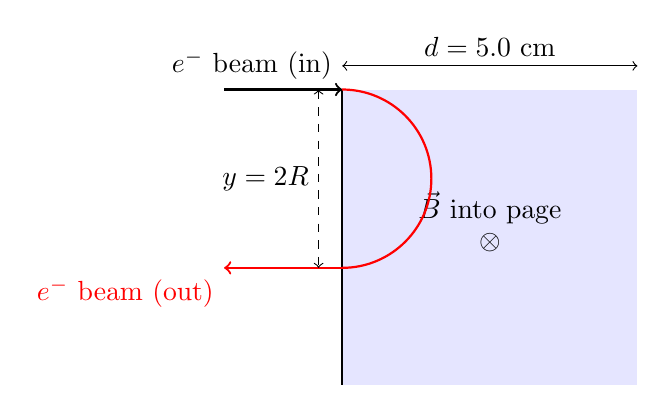
\begin{tikzpicture}[scale=1.5]
    % Define dimensions based on the problem
    \def\fieldwidth{2.5} % Represents 5.0 cm, scale is 2cm/unit
    \def\radius{0.755}   % Represents R=0.755 cm, but scaled for visibility
    \def\ydisp{\radius*2} % Represents y=2R

    % Draw the magnetic field region
    \fill[blue!10] (0,0) rectangle (\fieldwidth, -2.5);
    \draw[<->] (0, 0.2) -- (\fieldwidth, 0.2) node[midway, above] {$d = 5.0$ cm};
    \draw[thick] (0,0) -- (0, -2.5); % Left edge of field
    \node at (1.25, -1) {$\vec{B}$ into page};
    \node at (1.25, -1.3) {$\otimes$};

    % Draw incoming electron beam
    \draw[->, thick] (-1,0) -- (0,0) node[above left] {$e^-$ beam (in)};

    % Draw the semi-circular path
    % The electron enters at (0,0), force is down, so it curves down and left.
    % Center of circle is at (0, -R). Path is a clockwise semi-circle.
    % The arc command starts at (0,0) and draws an arc from 90 deg to -90 deg with radius R.
    \draw[thick, red] (0,0) arc (90:-90:\radius);

    % Draw outgoing beam
    \draw[->, thick, red] (0, -\ydisp) -- (-1, -\ydisp) node[below left] {$e^-$ beam (out)};

    % Add labels for displacement
    \draw[<->, dashed] (-0.2, 0) -- (-0.2, -\ydisp) node[midway, left] {$y = 2R$};
\end{tikzpicture}
\end{center}

\subsubsection*{Explanation}
First, we find the electron's speed by equating kinetic energy gained to electrical potential energy lost ($KE=eV$). Then, inside the magnetic field, the electrons follow a circular path with radius $R = \frac{m_ev}{eB}$. Since the calculated radius ($R=0.755$ cm) is smaller than the width of the field ($d=5.0$ cm), the electron completes a semi-circle and exits on the same side it entered. The vertical displacement will therefore be equal to the diameter of the circular path ($2R$).

\subsubsection*{Solution}
\begin{enumerate}
    \item \textbf{Find the electron's speed ($v$):}
    \begin{equation*}
        v = \sqrt{\frac{2eV}{m_e}} = \sqrt{\frac{2(1.60 \times 10^{-19} \text{ C})(500 \text{ V})}{9.11 \times 10^{-31} \text{ kg}}} \approx 1.326 \times 10^7 \text{ m/s}
    \end{equation*}
    \item \textbf{Calculate the radius of the circular path ($R$):}
    \begin{equation*}
        R = \frac{m_e v}{eB} = \frac{(9.11 \times 10^{-31} \text{ kg})(1.326 \times 10^7 \text{ m/s})}{(1.60 \times 10^{-19} \text{ C})(0.01 \text{ T})} \approx 0.00755 \text{ m} = 0.755 \text{ cm}
    \end{equation*}
    \item \textbf{Determine the vertical displacement ($y$):}
    The radius ($R=0.755$ cm) is smaller than the field width ($d=5.0$ cm). Therefore, the electron completes a full semi-circle and exits the field. The total vertical displacement is the diameter of the path.
    \begin{equation*}
        y = 2R = 2 \times 0.755 \text{ cm} = 1.51 \text{ cm}
    \end{equation*}
\end{enumerate}

\subsection{Problem 3: Bainbridge Mass Spectrometer}

\textbf{Question:} Singly ionized atoms of Lithium-6 ($m_6 = 9.988 \times 10^{-27}$ kg) and Lithium-7 ($m_7 = 1.165 \times 10^{-26}$ kg) are sent through a velocity filter with an electric field $E = 3.2 \times 10^5$ V/m and a magnetic field $B_1 = 0.8$ T. The ions that pass through undeflected then enter a second region with a uniform magnetic field $B_2 = 0.8$ T, which is perpendicular to their velocity.
(a) What is the speed of the ions that pass through the velocity filter?
(b) Calculate the radii of the semi-circular paths for the $^{6}$Li and $^{7}$Li isotopes in the second magnetic field.

\begin{center}
% THIS IS THE FINAL CORRECTED DIAGRAM
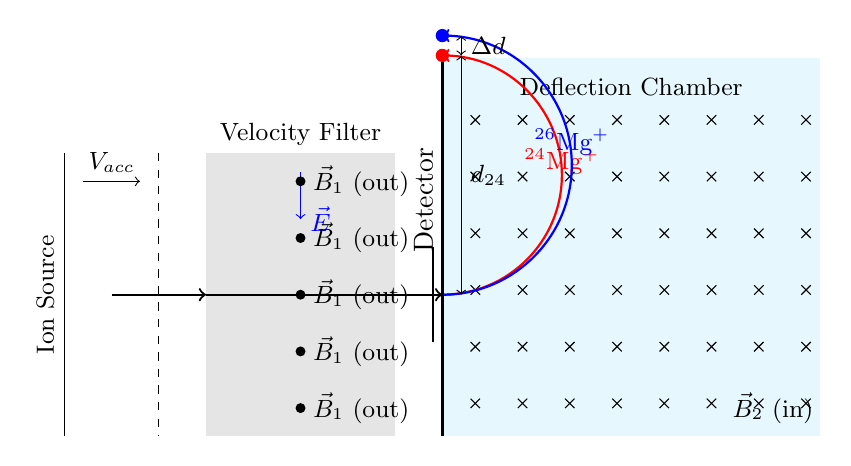
\begin{tikzpicture}[scale=1.2, font=\small]
    % Ion Source and Accelerator
    \draw (0,1.5) -- (0,-1.5);
    \draw[dashed] (1,1.5) -- (1,-1.5);
    \draw[->] (0.2, 1.2) -- (0.8, 1.2); \node at (0.5, 1.4) {$V_{acc}$};
    \node[rotate=90] at (-0.2, 0) {Ion Source};
    \draw[->, thick] (0.5, 0) -- (1.5, 0);

    % Velocity Filter
    \fill[gray!20] (1.5, -1.5) rectangle (3.5, 1.5);
    \node at (2.5, 1.7) {Velocity Filter};
    \draw[->, blue] (2.5, 1.3) -- (2.5, 0.8) node[right] {$\vec{E}$};
    \foreach \y in {-1.2, -0.6, 0, 0.6, 1.2}
        \fill (2.5, \y) circle (1.5pt) node[right=1pt] {$\vec{B}_1$ (out)};
    \draw[->, thick] (1.5, 0) -- (4, 0);
    \draw[thick] (3.9,-0.5) -- (3.9,0.5); % Slit
    \draw[thick] (4.1,-0.5) -- (4.1,0.5);

    % Deflection Chamber
    \fill[cyan!10] (4, -1.5) rectangle (8, 2.5);
    \node at (6, 2.2) {Deflection Chamber};
    % B2 field into page (correct for upward force)
    \foreach \x in {4.3, 4.8, 5.3, 5.8, 6.3, 6.8, 7.3, 7.8}
        \foreach \y in {-1.2, -0.6, 0, 0.6, 1.2, 1.8}
            \draw (\x, \y) -- ++(0.1, 0.1) (\x, \y) ++ (0.1, 0) -- ++(-0.1, 0.1) node[above right=1pt, color=cyan!50!black] {};
    \node at (7.5, -1.2) {$\vec{B}_2$ (in)};

    % Paths (Corrected to curve UP and land on the vertical detector)
    \def\rTwentyFour{1.266} % Scaled radius for Mg-24
    \def\rTwentySix{1.371}  % Scaled radius for Mg-26
    \draw[->, thick, red] (4, 0) arc (-90:90:\rTwentyFour); \node[red, above] at (4+\rTwentyFour, \rTwentyFour-0.1) {${}^{24}$Mg$^{+}$};
    \draw[->, thick, blue] (4, 0) arc (-90:90:\rTwentySix); \node[blue, above] at (4+\rTwentySix, \rTwentySix) {${}^{26}$Mg$^{+}$};

    % Detector
    \draw[very thick] (4, -1.5) -- (4, 2.5);
    \node[rotate=90, font=\normalsize] at (3.8, 1) {Detector};
    % Annotations for landing spots
    \coordinate (L24) at (4, 2*\rTwentyFour);
    \coordinate (L26) at (4, 2*\rTwentySix);
    \fill[red] (L24) circle (2pt);
    \fill[blue] (L26) circle (2pt);
    \draw[<->] (4.2, 0) -- (4.2, 2*\rTwentyFour) node[midway, right]{$d_{24}$};
    \draw[<->] (4.2, 2*\rTwentyFour) -- (4.2, 2*\rTwentySix) node[midway, right]{$\Delta d$};
\end{tikzpicture}
\end{center}

\subsubsection*{Explanation}
1. \textbf{Velocity Filter:} Only ions where the electric force ($F_E=qE$) balances the magnetic force ($F_B = qvB_1$) pass through undeflected. This determines the speed $v = E/B_1$.
2. \textbf{Separation Chamber:} The magnetic force ($F_B = qvB_2$) provides centripetal force for an upward circular path (by Right-Hand Rule: v is right, B is in, F is up). The radius $r = mv/qB_2$ depends on mass, separating the isotopes.

\subsubsection*{Solution}
\begin{enumerate}
    \item[(a)] \textbf{Find the speed of the ions ($v$):}
    \begin{align*}
        qE &= qvB_1 \\
        v = \frac{E}{B_1} &= \frac{3.2 \times 10^5 \text{ V/m}}{0.8 \text{ T}} = 4.0 \times 10^5 \text{ m/s}
    \end{align*}
    \item[(b)] \textbf{Calculate the radii of the paths ($r_6$ and $r_7$):}
    The charge $q$ is $+e = 1.60 \times 10^{-19}$ C.
    \begin{itemize}
        \item \textbf{$^{6}$Li:} $r_6 = \frac{m_6 v}{eB_2} = \frac{(9.988 \times 10^{-27})(4.0 \times 10^5)}{(1.60 \times 10^{-19})(0.8)} \approx 0.0312 \text{ m} = 3.12 \text{ cm}$
        \item \textbf{$^{7}$Li:} $r_7 = \frac{m_7 v}{eB_2} = \frac{(1.165 \times 10^{-26})(4.0 \times 10^5)}{(1.60 \times 10^{-19})(0.8)} \approx 0.0364 \text{ m} = 3.64 \text{ cm}$
    \end{itemize}
\end{enumerate}

\subsection{Problem 4: Oscillating Current Loop}

\textbf{Question:} A circular coil with 50 turns, a radius of 10 cm, and carrying a current of 2.0 A is placed in a uniform magnetic field of 0.25 T. The coil is pivoted about an axis that lies in the plane of the coil and passes through its center. A torsional spring with spring constant $\kappa = 0.50$ N·m/rad is attached to the pivot. In the equilibrium position, the plane of the coil is perpendicular to the magnetic field. The coil is rotated by 60 degrees from its equilibrium position and released from rest.
(a) What is the magnitude of the initial magnetic torque on the loop?
(b) What is the effective torsional constant for small oscillations around the equilibrium point?

\subsubsection*{Explanation}
When the coil is displaced, both the B-field and the spring exert a restoring torque. The total restoring torque is $\tau_{net} = \tau_B + \tau_s$. For small angles, we can approximate $\sin\theta \approx \theta$, and the net torque becomes proportional to $-\theta$, defining an effective torsional constant.

\subsubsection*{Solution}
\begin{enumerate}
    \item[(a)] \textbf{Calculate initial magnetic torque ($\tau_{B, initial}$):}
    \begin{itemize}
        \item Magnetic dipole moment $\mu = NIA = 50(2.0)\pi(0.10)^2 = 3.14 \text{ A·m}^2$.
        \item Initial angle $\theta = 60^\circ$.
        \begin{equation*}
            \tau_{B, initial} = \mu B \sin\theta = (3.14)(0.25)\sin(60^\circ) \approx 0.68 \text{ N·m}
        \end{equation*}
    \end{itemize}
    \item[(b)] \textbf{Find the effective torsional constant ($k_{eff}$):}
    \begin{itemize}
        \item The net restoring torque is $\tau_{net} = -(\mu B \sin\theta + \kappa\theta)$.
        \item For small angles $\theta$ in radians, $\sin\theta \approx \theta$.
        \begin{equation*}
            \tau_{net} \approx -(\mu B + \kappa)\theta
        \end{equation*}
        \item The effective torsional constant is the coefficient of the $-\theta$ term.
        \begin{align*}
            k_{eff} &= \mu B + \kappa \\
            &= (3.14)(0.25) + 0.50 \\
            &= 0.785 + 0.50 = 1.285 \text{ N·m/rad}
        \end{align*}
    \end{itemize}
\end{enumerate}

\subsection{Problem 5: Thermionic Emission and Magnetic Fields}
\textbf{Question:} Electrons are emitted from a hot filament with negligible initial speed and are accelerated through a potential difference of 2.0 kV. They then enter a uniform magnetic field of $4.0 \times 10^{-3}$ T, moving perpendicular to the field lines.
(a) What is the speed of the electrons as they enter the magnetic field?
(b) What is the radius of the circular path they follow inside the field?

\subsubsection*{Explanation}
First, use conservation of energy ($KE = eV$) to find the velocity of the electrons after acceleration. Then, use the formula for the radius of a charged particle's circular path in a magnetic field, $R = \frac{mv}{qB}$, derived by equating the magnetic force to the centripetal force.

\subsubsection*{Solution}
\begin{enumerate}
    \item[(a)] \textbf{Find the speed of the electrons ($v$):}
    \begin{align*}
        \frac{1}{2}m_e v^2 &= eV \\
        v = \sqrt{\frac{2eV}{m_e}} &= \sqrt{\frac{2(1.60 \times 10^{-19} \text{ C})(2000 \text{ V})}{9.11 \times 10^{-31} \text{ kg}}} \\
        &\approx 2.65 \times 10^7 \text{ m/s}
    \end{align*}
    \item[(b)] \textbf{Find the radius of the path ($R$):}
    \begin{align*}
        evB &= \frac{m_e v^2}{R} \\
        R = \frac{m_e v}{eB} &= \frac{(9.11 \times 10^{-31} \text{ kg})(2.65 \times 10^7 \text{ m/s})}{(1.60 \times 10^{-19} \text{ C})(4.0 \times 10^{-3} \text{ T})} \\
        &\approx 0.0377 \text{ m} \quad \text{or} \quad 3.77 \text{ cm}
    \end{align*}
\end{enumerate}

% --- END OF NEWLY INSERTED PROBLEMS ---

\end{document}